%
% teil2.tex -- Harmonische Systeme und Rauschen
%
% (c) 2023 Lukas Reitemeier, OST Ostschweizer Fachhochschule
%
% !TEX root = ../../buch.tex
% !TEX encoding = UTF-8
%

\section{Rauschen\label{brown:Rauschen}}
\rhead{Implikationen}

Um dem Thema des Buches gerecht zu werden und dieses Kapitel einzugliedern, kann die harmonische Analysis als essenzielles Werkzeug betrachtet werden. So ist zum Beispiel die \textit{Fast Fourier Transform (FFT)} eine wichtige Methode, um periodische Signale von Rauschen zu unterscheiden. So kann bezüglich der Intensität der auftretenden Frequenzen und der Verteilung der Amplituden im Frequenzspektrum, also deren Leistungsdichte, charakterisiert werden. 
So können mittels harmonischer Analysis Filter entwickelt werden, welche ein Signal von Rauschen befreien. Für gewisse Anwendungen ist es auch möglich, mit hochfrequent überlagerten Schwingungen, Rauschen zu simulieren. Durch die Analyse von Systemantworten auf verschiedene harmonische Anregungen, kann eine Aussage getroffen werden, wie ein System auf Rauschen --- also eine zufällige konstante Störung --- reagieren würde. 

\begin{figure}
	\centering
	\begin{minipage}{0.48\textwidth}
		\centering
		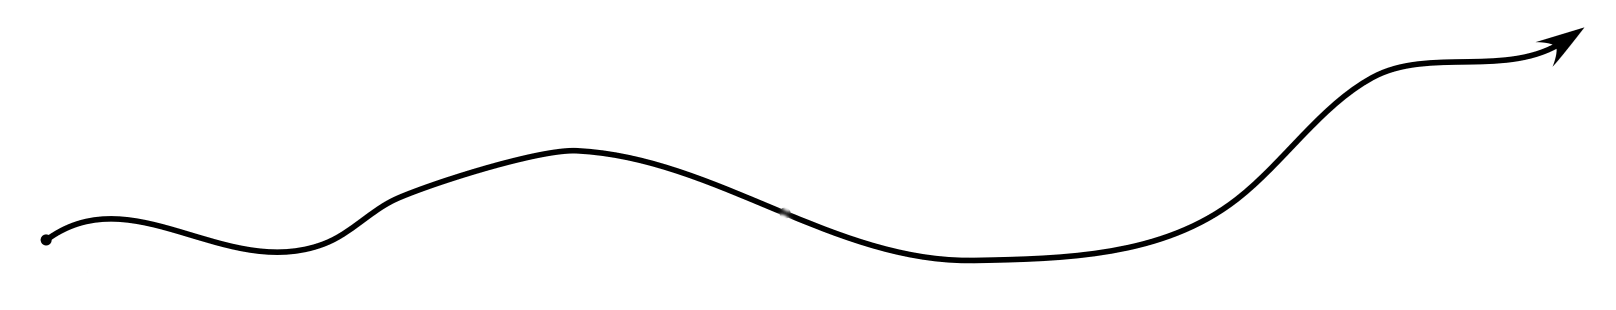
\includegraphics[width=\textwidth]{papers/brown/images/idealSignal2.png}
		\caption{Ideales Signal}
		\label{idealSignal}
	\end{minipage}
	%\hspace{0.05\linewidth}
	\begin{minipage}{0.48\textwidth}
		\centering
		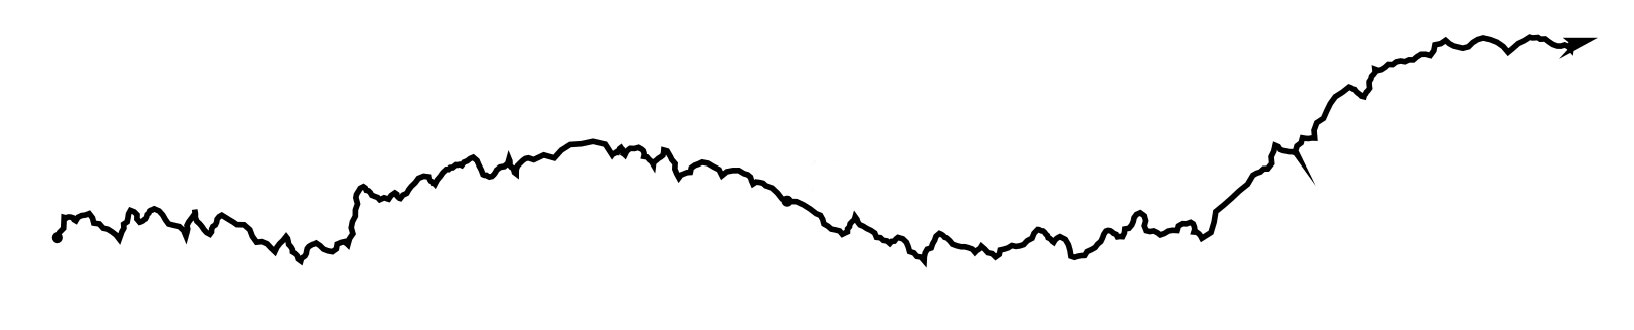
\includegraphics[width=\textwidth]{papers/brown/images/realSignal2.png}
		\caption{Reales Signal}
		\label{realSignal}
	\end{minipage}
\end{figure}

%Problematisch dabei kann sein, dass je nach Definition und Anwendung \textit{echtes Rauschen} weder vorhersagbar sein sollte, noch Information beinhalten.

%All diese Beispiele basieren auf Methoden der harmonischen Analysis, um den Bogen zur Anfangsbemerkung dieses Kapitels zu schliessen.


\subsection{Was ist Rauschen?\label{brown:Rauschen:Arten}}

Rauschen ist in vielen technischen und wissenschaftlichen Disziplinen ein wichtiger Faktor, so kann es auch in verschiedenen Kontexten unterschiedlich definiert werden. In der Signal- und Kommunikationstechnik ist Rauschen als ungewollte Störung eines Signals definiert. Ein perfektes, ungestörtes Signal, wie es in Abbildung \ref{idealSignal} dargestellt ist, gibt es nur in der Theorie. In der Realität sind alle Signale von Rauschen behaftet, wie in der Abbildung \ref{realSignal} dargestellt. Eine solche Störung kann auf einem deterministischen Zusammenhang beruhen oder rein zufälliger Natur sein. Zum Beispiel kann bei elektronischen Messungen durch das Magnetfeld von Stromkabeln eine Störung hervorgerufen werden, dies wäre eine deterministische Störungen (konstant 50 Hz Wechselstrom). Es gibt aber auch rein zufällige Störungen, wie zum Beispiel durch kosmische Teilchen, welche einen Empfänger oder Messgerät beeinflussen können. Wird ein Signal konstant von Störungen beeinflusst, kann von Rauschen gesprochen werden. Mathematisch können unterschiedliche Arten von Rauschen unterschieden werden \cite{werner2008signale}, einige der wichtigsten sind folgende: 


\begin{definition}
{\em Weisses Rauschen:}
Ein Signal mit zufälligen Änderungen, welches eine konstante spektrale Leistungsdichte über alle Frequenzen hinweg aufweisst (alle Frequenzkomponenten sind mit gleicher Intensität vertreten).
\end{definition}

Das Rauschen wird als ``weiss'' bezeichnet, analog zu weissem Licht, bei dem alle Farben des sichtbaren Spektrums überlagert sind. Es ist aber anzumerken, dass weisses Licht keine konstante Leistungsdichte im Spektrum aufweisst. In der Zeitdomäne ist das weisse Rauschen ein unkorreliertes Signal. Ein Beispiel dafür ist das Rauschen von Radios, wenn die Frequenz nicht korrekt eingestellt ist. Dies wird ausgelöst durch Störeinflüsse, wie zum Beispiel: Elektrische Interferenzen, kosmische Einflüsse oder auch Blitzentladungen.


\begin{definition}
	{\em Rosa Rauschen:}
	Ein Signal mit zufälligen Änderungen, dessen Amplituden invers proportional zur Frequenz $ ~1/f $  abnehmen. In der Elektronik wird der Abfall der Leistungsdichte mit 3 \text{dB} pro Oktave charakterisiert.
\end{definition}

 Der Begriff ``Rosa'' ist auch eine Analogie zum sichtbaren Licht, bei dem tiefere Frequenzen eher rötlich erscheinen und überlagert mit Weiss (weisses Rauschen), Rosa ergeben. Um bei einem hörbaren Beispiel zu bleiben: Rosa Rauschen klingt als Schall ausgewogener und ``weicher'' als weisses Rauschen. Dies, da unangenehme hohe Frequenzen abgeschwächt werden und somit weniger dominant sind.

\begin{definition}
	{\em Braunes Rauschen (Brownsches Rauschen):}
	Ein Signal mit zufälligen Änderungen, dessen Amplituden invers quadratisch zur Frequenz $ ~1/f^2 $ abnehmen. In der Elektronik wird der Abfall der Leistungsdichte mit 6 \text{dB} pro Oktave charakterisiert.
\end{definition}

\textit{Braun} bezieht sich hier nicht auf eine Farbe, sondern ist Robert Brown gewidmet. Denn die Brownsche Modekühlbewegung entspricht diesem Rausch-Typ, da sich die beobachteten trägen Moleküle mit zunehmender Frequenz verstärkt gegenseitig behindern.

\begin{definition}
	{\em Gaussisches Rauschen:}
	Ein Signal mit zufälligen Änderungen, dessen Amplituden im Frequenzspektrum eine Normalverteilung (Gaussverteilung) um eine zentrale Frequenz aufweisen. Demzufolge kann Gaussisches Rauschen über zwei Parameter charakterisiert werden: den Mittelwert und die Varianz.
\end{definition}

Gaussisches Rauschen ist ein häufiges Artefakt in digitalen Bildern und daher von besonderer Bedeutung in der digitalen Bildverarbeitung. Die charakteristische ``Körnigkeit'' des Rauschens in einem Bild kann über eine zentrale Frequenz charakterisiert werden.

\begin{definition}
	{\em Impulsrauschen:}
	Ein Signal mit zufälligen kurzzeitigen Spitzen oder Abfälle der Signalintensität, also diskontinuierlichen skalierten Impulsen. 
\end{definition}

Im Frequenzspektrum äussern sich die Impulse über einen breiten Bereich, ähnlich zur Fourier-Transformation eines Dirac-Impulses. Ein idealer Dirac-Impuls im Zeitbereich stellt im Frequenzbereich einen konstanten Wert über alle Frequenzen dar.
In der digitalen Bildverarbeitung ist diese Art von Rauschen als \textit{salt} \& \textit{pepper} bekannt. Dabei nehmen einzelne Pixel sporadisch extreme Werte an, entweder extrem dunkel (pepper) oder extrem hell (salt). Diese Pixel sind auf dem Bild leicht erkennbar und wirken ähnlich wie verstreute Salz- oder Pfefferkörner.


Natürlich kann noch zwischen vielen weiteren Typen unterschieden werden, doch auf diese wird nicht eingegangen.


%\begin{figure}
%	\centering
%	\begin{minipage}{0.48\textwidth}
%		\centering
%		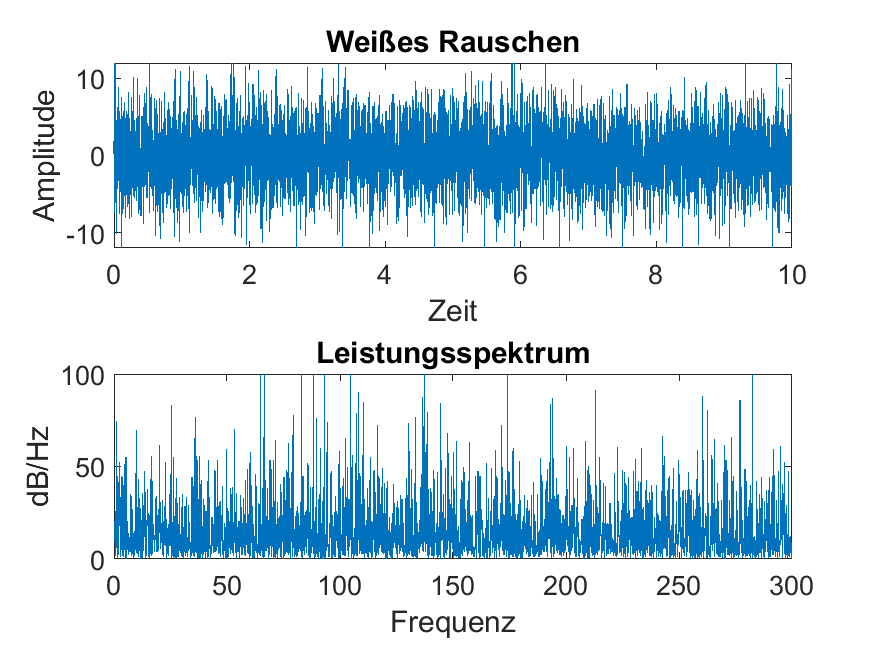
\includegraphics[width=\linewidth]{papers/brown/images/weissesRauschen-FFT.png}
%		\caption{Echtes weisses Rauschen}
%		\label{brown:weissesRauschenSignal}
%	\end{minipage}
%	%\hspace{0.05\linewidth}
%	\begin{minipage}{0.48\textwidth}
%		\centering
%		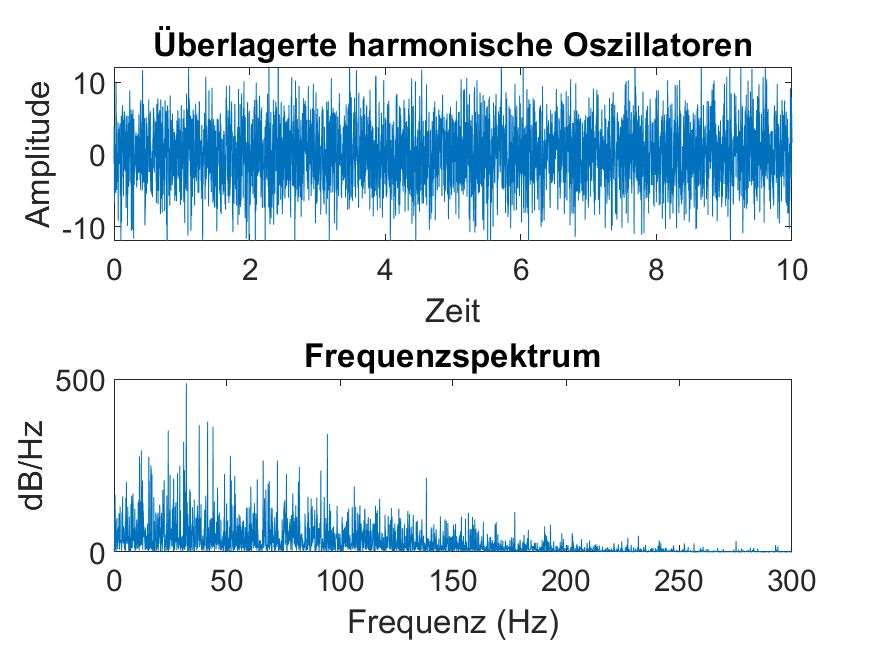
\includegraphics[width=\linewidth]{papers/brown/images/harmonischeOszillatoren-FFT.png}
%		\caption{Überlagerte harmonische Oszillatoren}
%		\label{brown:überlagerteSchwingungen}
%	\end{minipage}
%\end{figure}

\begin{figure}
	\centering
	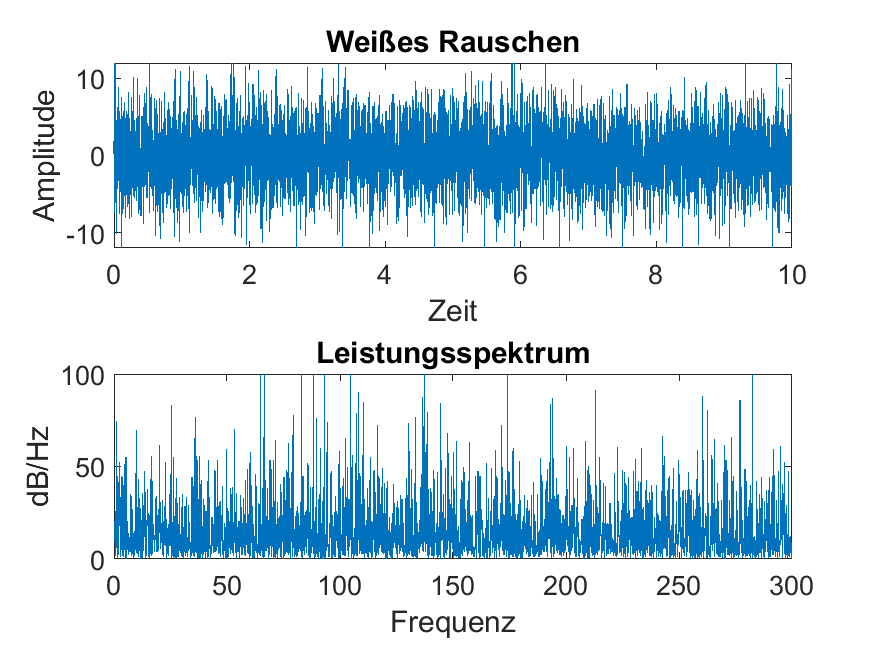
\includegraphics[width=0.8\textwidth]{papers/brown/images/weissesRauschen-FFT.png}
	\caption{Echtes weisses Rauschen}
	\label{brown:weissesRauschenSignal}
\end{figure}

\begin{figure}	
	\centering
	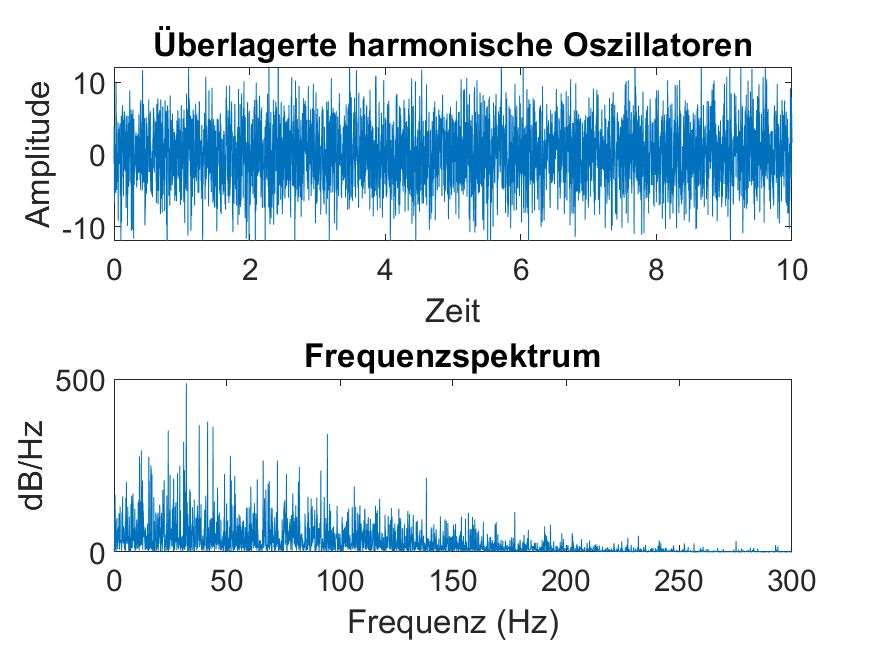
\includegraphics[width=0.8\textwidth]{papers/brown/images/harmonischeOszillatoren-FFT.png}
	\caption{Überlagerte harmonische Oszillatoren}
	\label{brown:überlagerteSchwingungen}
\end{figure}


Es gibt auch Signale die visuell wie Rauschen wirken, obwohl diese kaum von einer zufälligen Störungen behaftet sind. So zum Beispiel hochfrequente überlagerte Schwingungen oder auch aufmodulierte Signale. In der Nachrichtentechnik wird dies aus technischen Gründen gemacht, um zum Beispiel mehr Information über den selben Signalträger zu senden oder das Signale robuster zu übertragen. In den Abbildungen~\ref{brown:weissesRauschenSignal} und~\ref{brown:überlagerteSchwingungen} sind zwei Signale aufgetragen, eines stellt echtes stochastisches Rauschen dar, das andere besteht aus vielen hochfrequenten überlagerten Schwingungen. Dieses Beispiel soll verdeutlichen, dass es nicht reicht, nur den zeitlichen Verlauf eines Signals zu betrachten. So könnte man fälschlicherweise die Signale als ähnlich erachten --- eine krasse Täuschung, welche sich im Frequenzspektrum klar zeigt. 



\subsection{Rauschen mittels Wiener-Prozess\label{brown:Rauschen:RandomWalkWiener}}

Um Rauschen zu modellieren, muss als Grundlage ein stochastischer Prozess definiert werden. Zwei weit verbreitete Konzepte dabei sind der \textit{random walk} und der \textit{Wiener-Prozess}.

\begin{definition}\textbf{Random Walk:}
	\label{randomWalk}
	Bei einem Random Walk beginnt man an einem Ausgangspunkt (normalerweise 0) und macht bei jedem Zeitschritt einen zufälligen Schritt vor oder zurück. Oft dient dazu die Binominalverteilung, wobei auch asymmetrische Verteilungen verwendet werden können. Die Schrittlänge und Richtung kann ebenfalls durch eine unabhängige Wahrscheinlichkeitsverteilung bestimmt werden, wobei meist eine konstante Schrittlänge angenommen wird. Dieses Verfahren zeichnet sich durch eine einfache numerische Implementation aus, da es per Definition schon diskret ist.
\end{definition}

\begin{definition}\textbf{Wiener-Prozess:}
	\label{wienerprozess}
	Der Wiener-Prozess ist ein kontinuierlicher stochastischer Prozess, der mit dem Wert 0 startet und unabhängige normalverteilte Änderungen aufweisst. Speziell dabei ist, dass unabhängig von der verstrichenen Zeit der Erwartungswert stets dem Ausgangswert entspricht. Der Wiener-Prozess kann auch als Grenzwert eines Random Walks erachtet werden, sofern die Zeitschritte und Schrittgrössen gegen null gehen und der Prozess bei 0 startet.
\end{definition}

Beide Prozesse erfüllen die sogenannte \textit{Markov-Eigenschaft}, was bedeutet dass ihre zukünftige Entwicklung nur von ihrer aktuellen Position und nicht von ihrer vergangenen Geschichte abhängt.

Der Wiener-Prozess und die Brownsche Bewegung werden oft als Synonyme verwendet. Beides sind kontinuierliche stochastische Prozesse, wobei der Wiener-Prozess explizit nirgends differenzierbar ist und eher in der Mathematik zur Anwendung kommt.

Der Wiener-Prozess muss formal also folgende Eigenschaften erfüllen: 

\begin{enumerate}
	\item Der Startwert von $ t = 0 $ ist $ W(0) = 0 $.
	\item $ W(t_{1}) - W(t_{2}) $ ist eine normalverteilte Zufallsvariable mit Erwartungswert 0 und Varianz $ t_{1} - t_{2} $. Es ergibt sich folgender Zusammenhang: $ dW^2 = dt $.
	\item Zu jedem weiteren Zeitpunkt $ t_{n} $ ist die Zufalls-Variable unabhängig von allen vorhergehenden Werten (Markov-Eigenschaft) und nirgends differenzierbar.
\end{enumerate}


Genauer wird auf den Wiener-Prozess nicht eingegangen, da dieser ausführlich im Kapitel \textit{8.1 Modell für Rauschen: der Wiener-Prozess} des Buches \cite{brown:Differenzialgleichungen} vom Mathematischen Seminar über Differenzialgleichungen beschrieben wird.


Nun, da der Wiener-Prozess definiert ist, soll versucht werden weisses Rauschen zu simulieren. Dafür eignet sich der Wiener-Prozess perfekt, denn die Ableitung nach der Zeit
\begin{equation}
	\xi(t) = \frac{dW(t)}{dt}
\end{equation}
ergibt weisses Rauschen. Dies ist auch der Grund, weshalb der Wiener-Prozess als nicht differenzierbar definiert ist. Die Änderungen sind rein zufällig und normalverteilt, so ergibt sich ein gleichmässiges Frequenzspektrum der Änderungsraten. Es ist also keinerlei Information in den Änderungsraten enthalten.

%Da der in der Abbildung \ref{brown:1Dbrownian} dargestellte Börsen-Verlauf nichts anderes als der Wiener-Prozess mit Drift-Komponente ist, sollte weisses Rauschen durch dessen Differenzierung generiert werden können. In der Abbilung \ref{...} wurde das Frequenzspektrum des simulierten Börsenkurses berechnet. 

In der Abbildung \ref{brown:diffWienerFFT} ist die Simulation eines Wiener-Prozesses, also einer brownschen Bewegung, und dessen Frequenzspektrum aufgetragen. Der Unterschied zum simulierten Börsenkurs in der Abbildung \ref{brown:1Dbrownian} ist lediglich, dass keine absichtliche Drift-Komponente modelliert wurde. Man kann feststellen, dass die Leistungsdichte mit zunehmender Frequenz abnimmt. Dies bedeutet, dass tiefe Frequenzen sich im Signal stärker äussern als hohe, also mehr Energie beinhalten. Durch differenzieren der Brownschen Bewegung ergibt sich ein konstantes Frequenzspektrum. In der Zeitdomäne stellt das Signal ausschliesslich weisses Rauschen dar, wie in der Darstellung \ref{brown:diffWienerFFT} zu sehen ist.

%ToDo: Alles in eine Grafik und übereinander gross darstellen
%\begin{figure}
%	\centering
%		\centering
%		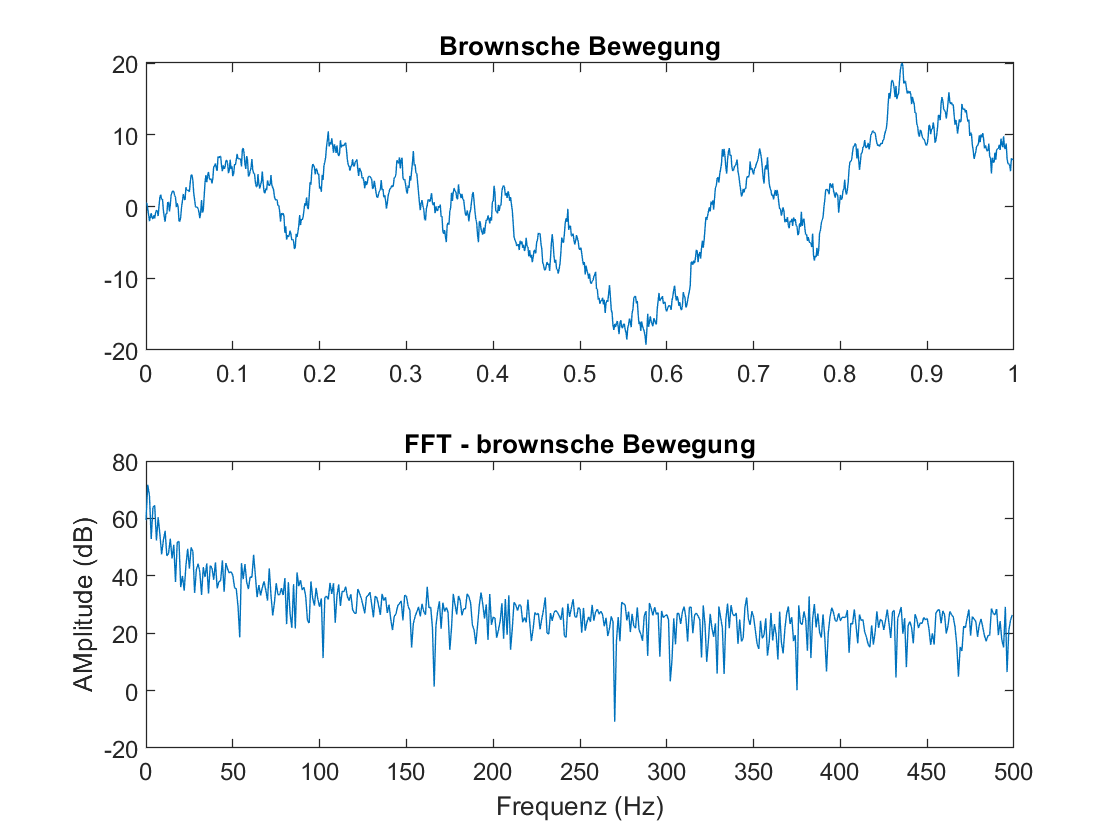
\includegraphics[width=\linewidth]{papers/brown/images/brownscheBewegungUndFFT.png}
%		\caption{Wiener-Prozess und Frequenzspektrum}
%		\label{brown:WienerProzessFFT}
%	\end{minipage}
%	%\hspace{0.05\linewidth}
%	\begin{minipage}{0.48\textwidth}
%		\centering
%		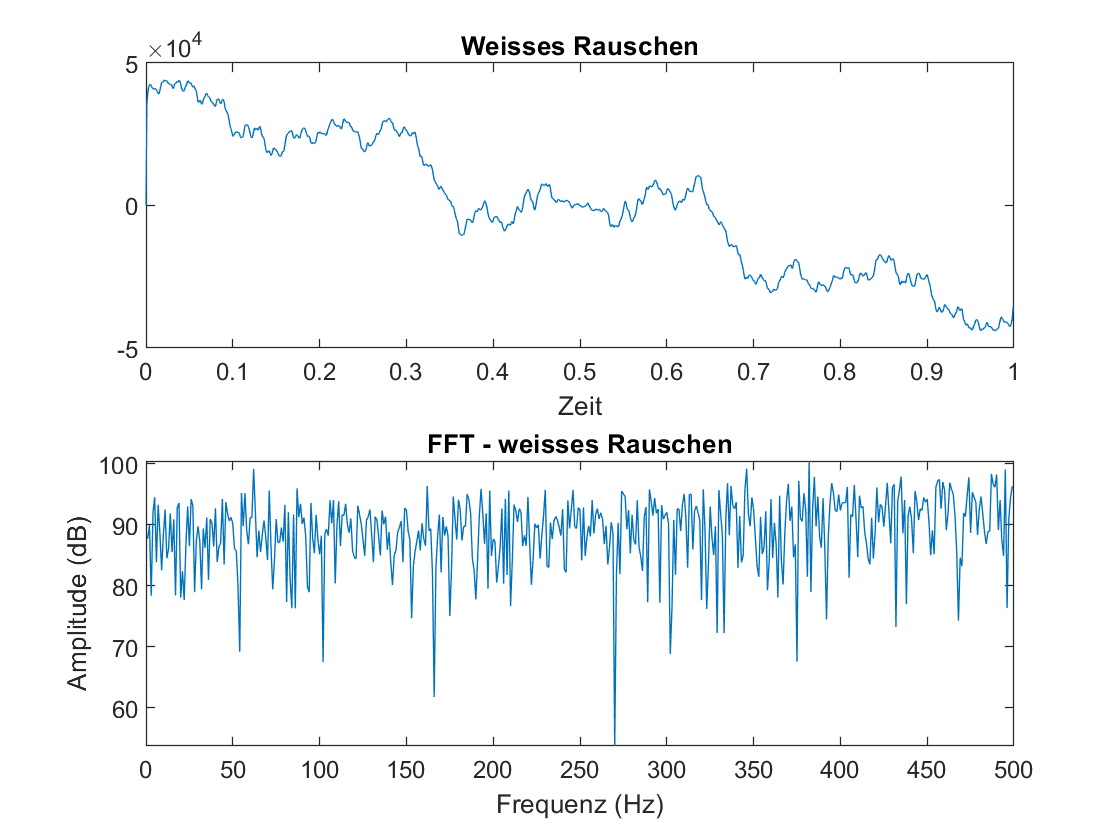
\includegraphics[width=\linewidth]{papers/brown/images/weissesRauschenDurchBrownUndFFT.png}
%		\caption{differenzierter Wiener-Prozess und Frequenzspektrum}
%		\label{brown:diffWienerFFT}
%	\end{minipage}
%\end{figure}

\begin{figure}
	\centering
	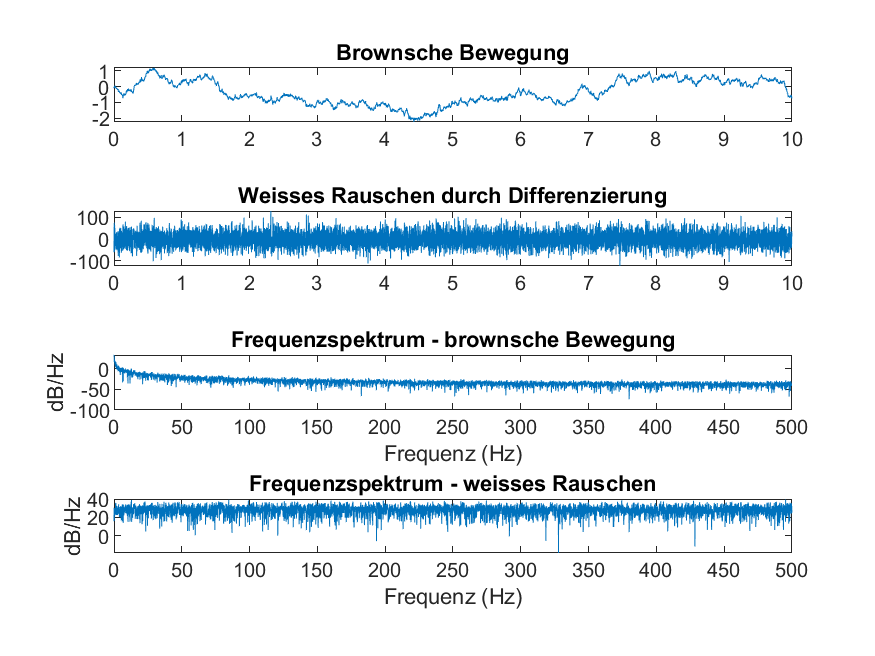
\includegraphics[width=0.95\textwidth]{papers/brown/images/weissesRauscheDurchBrown-timeDomain.png}
	\caption{Weisses Rauschen durch Differenzierung des Wiener-Prozess}
	\label{brown:diffWienerFFT}
\end{figure}


\subsection{Implikationen\label{brown:Rauschen:Implikationen}}

Beim Umgang mit Messdaten und empfangene Signalen ist die Problematik von Störungen und dessen Einfluss auf die berechneten Änderungsraten allgegenwärtig. Dies  kann zu falsch dekodierter Information und ungenauen Messergebnissen führen. Die einfachste Methode und häufig ein erster Schritt ist die Anwendung eines Tiefpass- oder Bandpassfilters. Dieser entfernt jedoch nicht nur störende Frequenzen, sondern auch ein Teil der im Signal enthaltenen Information. Die Anwendung eines gleitenden Mittelwertes lässt Störungen sich auf das Ganze Signal auswirken. Die ist speziell problematisch bei kurzzeitigen intensiven Störungen, wie dies bei Impulsrauschen der Fall ist. In solchen Fällen ist ein Medianfilter zu bevorzugen.

Eine weitere Schwierigkeit entsteht, wenn anhand von Messdaten ein Modell erstellt werden soll, welches das Verhalten der Messdaten widerspiegelt. Dabei kann es sein, dass das Rauschen als Teil des Systems identifiziert wird oder als rein externe Störung. Im einen Fall muss dann zwischen System und Rauschen unterschieden werden, im anderen Fall muss das System selbst Rauschen abbilden können.
% Absatz?

Ist ein System anhand einer gewöhnlichen Differenzialgleichung (DGL) gegeben, kann das Verhalten des Systems unter Berücksichtigung der Anfangsbedingungen vorhergesagt werden. Vom Anfangswert aus entwickelt sich die Funktion gemäss der Startbedingung und dem durch die DGL gegebenen Vektorfeld. In vielen Bereichen entspricht ein solch deterministisches System jedoch nicht der Realität und suggeriert eine Aussagekraft, welche sich nicht mit Beobachtungen deckt. Es gibt Systeme, welche stark auf kleine Störeinflüsse reagieren. Dies führt dazu, dass sich die Lösung einer DGL gegenüber der Realität, zum Beispiel durch Rauschen, nicht perfekt deckt oder das Resultat sogar komplett divergiert. Ein anschauliches Beispiel dafür ist das System
\begin{align}
	\frac{dx}{dt} &= -y \\
	\frac{dy}{dt} &= x^2 + y
	\label{brown:divergentEquation},
\end{align}
für welches in der Abbildung~\ref{brown:divergentAndConvergentSystem} zwei unterschiedliche Trajektorien im Vektorfeld eingezeichnet sind. In rot ist der Verlauf im Intervall  $ t = [0, 3] $ mit dem Startwert $ (-1.7, -1.4) $ aufgetragen und in grün mit dem Startwert $ (-1.8, -1.4) $.

\begin{figure}
	\centering
	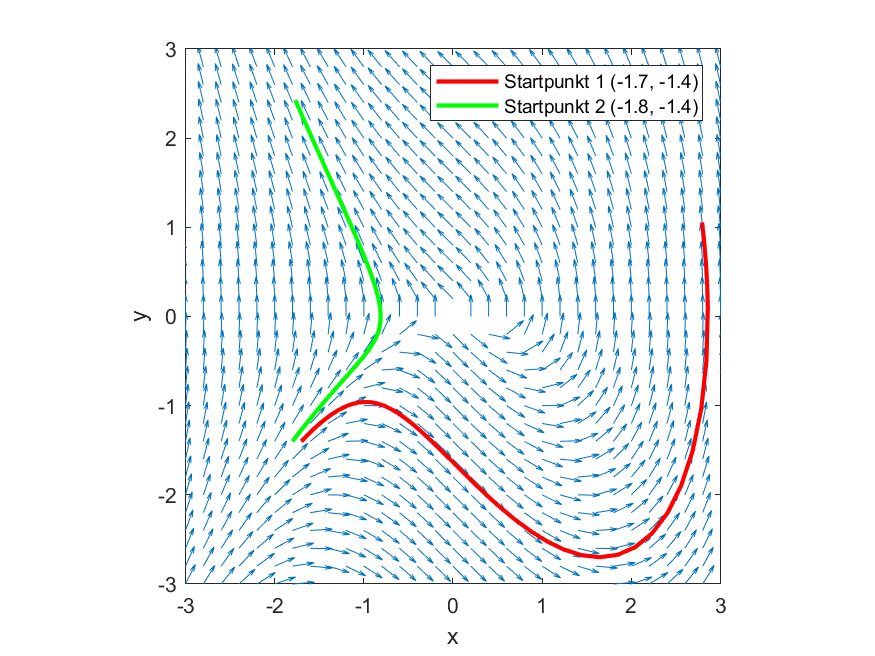
\includegraphics[width=0.95\textwidth]{papers/brown/images/divergentDGL.png}
	\caption{Vektorfeld mit zwei divergierenden Pfaden, trotz fast gleichem Startwert}
	\label{brown:divergentAndConvergentSystem}
\end{figure}

Dieses System veranschaulicht schön, wie sich eine kleine Variation der Startbedingung auf den Verlauf der Lösung auswirken kann. In diesem speziellen Fall konvergieren die Lösung zu einem späteren Zeitpunkt $ t $ wieder. Bedenkt man nun aber, dass eine solche Störung durch Rauschen herbeigeführt werden könnte, scheint es unsinnig, eine einzige fixe Lösung für ein solches System anzugeben --- zumindest nicht ohne auf die Aussagekraft der Lösung, unter Rauscheinfluss, hinzuweisen oder den Lösungsraum genauer zu spezifizieren.

Es gibt auch Systeme, welche bei kleinen Störungen aus einem stabilen Zustand in einen instabilen Zustand übergehen und komplett divergieren. In solchen Fällen kann es ein fataler Fehler sein, zufällige Störungen des Systems nicht zu berücksichtigen. Andere Systeme beinhalten selbst eine zufällige Komponente, welche nicht vernachlässigt werden soll.

Um diesem Umstand gerecht zu werden, kann man die Möglichkeit von zufälligen Störungen beim Aufstellen eines Modells miteinbeziehen. Anstatt eine fixe Lösung zum Zeitpunkt $ t $ anzugeben, kann man eine Wahrscheinlichkeitsverteilung über die verschiedenen möglichen Endzustände angeben --- et voilà, man hat den Lösungsraum einer stochastische Differenzialgleichung (SDGL).
